\usepackage{acronym}
\usepackage{afterpage}
\usepackage[noend]{algpseudocode}
\usepackage{appendix}
\usepackage{booktabs} % improving tables
\usepackage{enumitem}
\usepackage{epigraph}
\usepackage{include/epipart}
\usepackage{float}
\usepackage[margin = 1.2in]{geometry} % change the page margins
\usepackage{textcomp} % To avoid warnings in gensymb
\usepackage{gensymb} % for generic symbols
\usepackage{graphicx} % to use \includegraphics
\usepackage{hyperref} % adding urls using \url
\usepackage[utf8]{inputenc} % makes sure other characters than ASCII can be used
\usepackage{listings} % to add code snippets
\usepackage{multicol} % use multiple columns in text
\usepackage{parskip} % makes sure that a line is skipped after every paragraph
\usepackage{pifont} % For checkmark and cross mark
\usepackage{setspace} % set spacing in paragrahs like contents
\usepackage{subcaption} % for caption of subfigures
\usepackage{tikz} % for graphics, also build front cover using tikz
\usepackage{titlesec, color}
\usepackage[textsize=footnotesize]{todonotes} % placing todo notes and summarizing them at start of document
\usepackage{wrapfig}

%% Todonots setting
\presetkeys{todonotes}{inline, bordercolor=orange, backgroundcolor=blue!10, linecolor=black}{}

%% Bibliography style
\bibliographystyle{include/tudelft-report}

%% Change font to sans-serif
\renewcommand{\familydefault}{\sfdefault}

%% Folder with figures
\graphicspath{{figure/}}

%% Epigraph size
\setlength{\epigraphwidth}{0.45\textwidth}

%% No line-breaking
\hyphenpenalty=10000

%% Captions always centered
\captionsetup{justification=centering}

%% Symbols to link dependent variables
\newcommand{\performance}{$\clubsuit$}
\newcommand{\trust}{$\diamondsuit$}
\newcommand{\participant}{$\odot$}
\newcommand{\SA}{$\spadesuit$}
\newcommand{\satisfaction}{$\heartsuit$}
\newcommand{\protocol}{$\star$}

%% Text lay-out
% Customize chapter style
\titleformat
{\chapter} % command
[hang] % shape
{\bfseries \LARGE \raggedright} % format
{\thechapter \hspace{5pt} \textcolor{cyan} {$|$} } % label
{0pt}
{\bfseries \LARGE \raggedright} % before-code
[] % after-code

\titlespacing
{\chapter}
{30pt} % Left
{-30pt} % Top
{5pt} % Bottom
%%  Hyperlink colors
\hypersetup{ %setup hyperlinks
    colorlinks,
    citecolor=black,
    filecolor=black,
    linkcolor=black,
    urlcolor=black
}

\setlength{\parindent}{0pt}

%% Line spacing
\renewcommand{\baselinestretch}{1.35} 

%% Tikz settings
\usetikzlibrary{arrows,shapes,positioning,shadows,trees}


%% Front cover, blank page, title page command
\newcommand{\emptyDoublePage}{
	\newpage
	\phantom{-}
	\newpage
}

\newcommand{\addCoverPage}{
	%% Create an empty page for cover.
	\clearpage
	\thispagestyle{empty}

 	%% Building cover
	\begin{tikzpicture}[remember picture,overlay]
		\node (picture) at (current page.center)
		{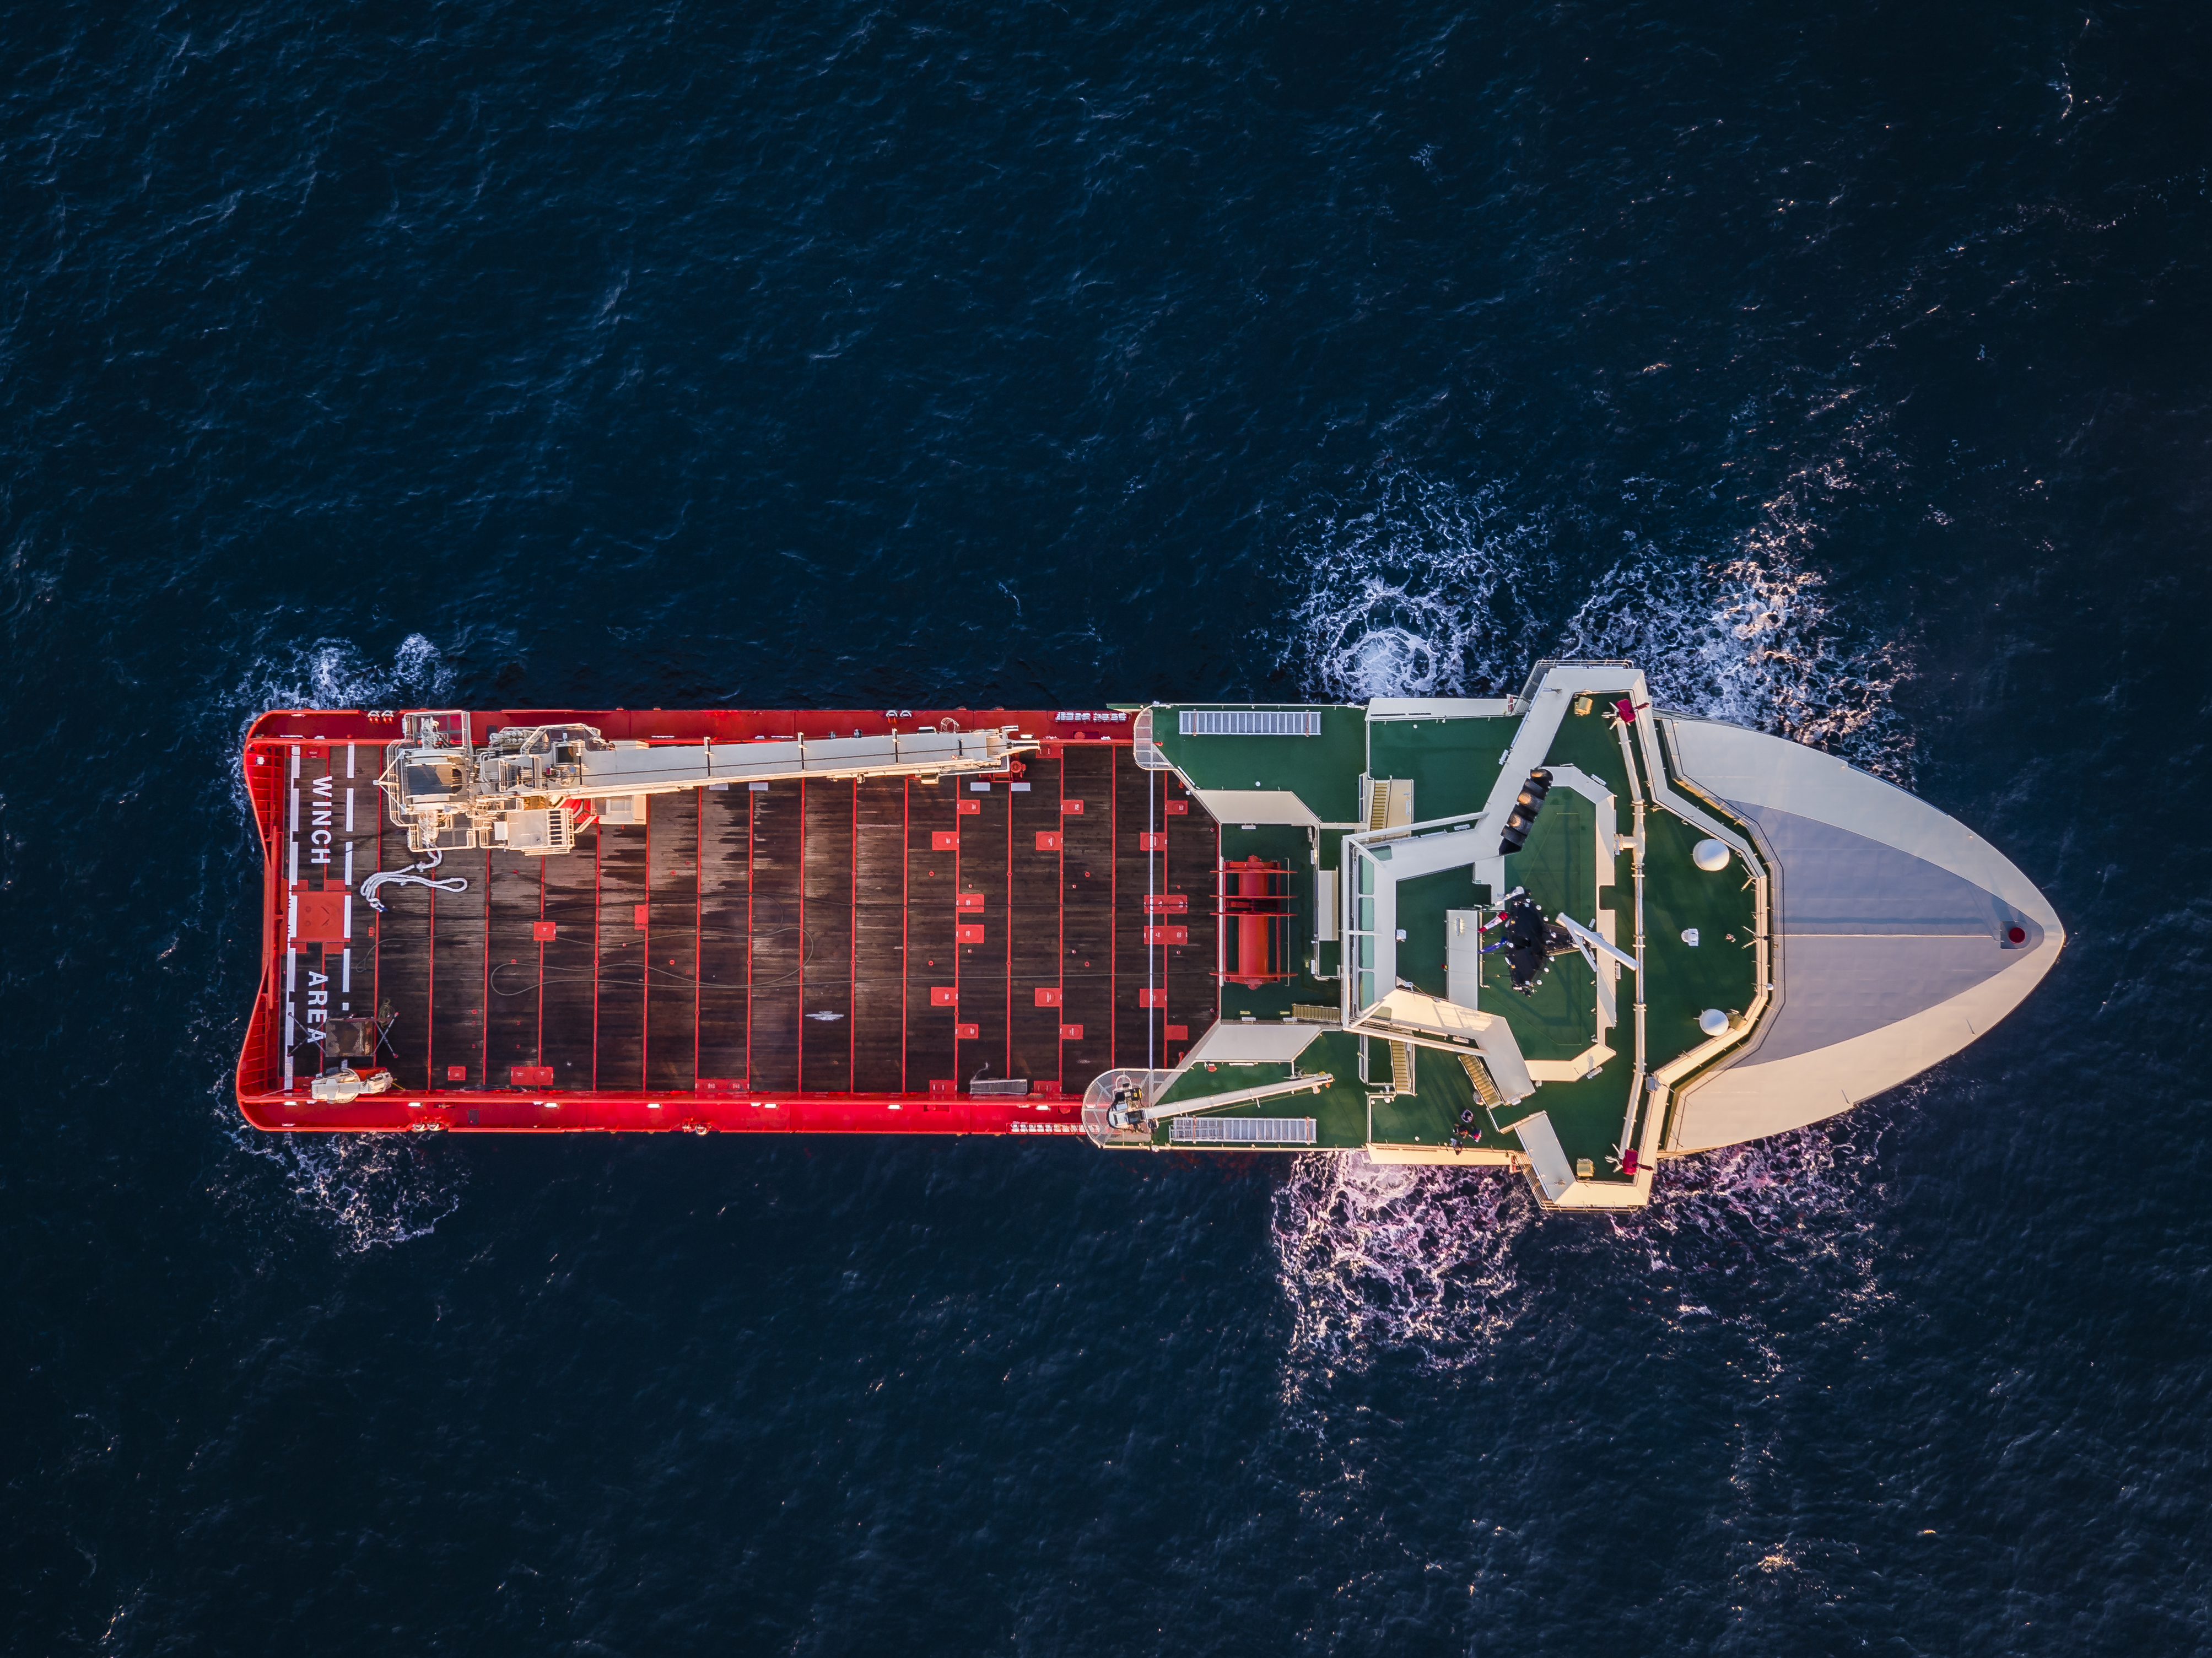
\includegraphics[height=\paperheight, keepaspectratio]{cover_PSV_5000_top.jpg}};
		
		\node (white-glow) at (current page.center) [fill = white, minimum width = \paperwidth, minimum height = \paperheight, opacity = 0.15]{};
		
		\node (title-box-bg) at (current page.east) [fill = gray, minimum width=.5\paperwidth, minimum height=7cm, fill opacity = 0.85, xshift=-.3\paperwidth, yshift=-5cm, text=white] {};
		
		\node (title-box) at (current page.east) [minimum width=.5\paperwidth, minimum height=7cm, align=left, xshift=-.3\paperwidth, yshift=-5cm, text=white] {
			\hspace{.5cm}
			\huge{MSc Thesis Report} \\ \\
			\Large{Manoeuvrability and communication} \\
			\Large{requirements for safe operation when} \\
			\Large{manned and unmanned vessels meet} \\ \\
			Ingmar Wever \\
			\today
			
		};
	
		\node (black-bar) [fill = black, minimum width=.5\paperwidth, minimum height=0.2cm, yshift = -3.4cm, fill opacity = 0.7] at (title-box){};
		
		\node (cyan-bar) [fill = cyan, minimum width=.5\paperwidth, minimum height=0.2cm, yshift = -3.6cm, fill opacity = 0.7] at (title-box){};
		
		\node (white-bar) [fill = white, minimum width=.5\paperwidth, minimum height=1.5cm, yshift = -4.5cm, fill opacity = 0.95] at (title-box){
		
			\includegraphics[height=1.3cm, keepaspectratio]{TU_Delft_logo_RGB.png}
			\hspace{.8cm}
			\includegraphics[height=.8cm, keepaspectratio]{Damen_logo.png}
		};
	
		
	\end{tikzpicture}
}

\newcommand{\addEmptyPage}{
	%% Create empty page for two-sided printing
	\clearpage
	\setcounter{page}{0}
	\thispagestyle{empty}
	\vspace*{6cm}
	\begin{center}
		This page is intentionally left blank.
		
		\tiny{(Except for the above line.)}

	\end{center}
	\todo{Titels begeleiders and graduation date}
}

\newcommand{\addTitlePage}{
	\begin{titlepage}
	
	%% Title page
	\newpage
	
	\centering
	\Large
	\vspace*{1cm}
	Thesis Report for the degree of \\ 
	MSc Marine Technology and MSc Computer Science\\
	\vspace{1cm}
	\begin{spacing}{2}
		\begin{Huge}
			Manoeuvrability and communication requirements for safe operation when manned and unmanned vessels meet
		\end{Huge}
	\end{spacing}
	\large
	\vspace{1cm}	
	by Ingmar Wever
	at Damen Shipyards and TU Delft
	
	\today
	
	\vspace{1.5cm}
	\footnotesize
	This thesis (SDPO.18.048.m) is classified as confidential in accordancewith the general conditions for projects performed by the TU Delft. 
	
	\vspace{3cm}
	\normalsize
	\begin{tabular}{lll}
		Student: & Ingmar Wever & 4161041 \\
		Project duration: & \multicolumn{2}{l}{September 2017 -- November 2018} \\
		& & \\
		Supervisors: & Dr.ir. Robert Hekkenberg & TU Delft, Ship Design \\
		& Prof.Dr. Mark Neerincx & TU Delft, Interactive Intelligence \\
		& Toine Cleophas & Damen Shipyards, R\&D \\
		Committee members: & Peter de Vos MSc. & TU Delft, Marine Engineering \\
		& Dr.ir. Willem-Paul Brinkman & TU Delft, Interactive Intelligence \\
	\end{tabular}

	\end{titlepage}
}
	